\documentclass[conf]{new-aiaa}
%\documentclass[journal]{new-aiaa} for journal papers
\usepackage[utf8]{inputenc}

\usepackage{graphicx}
\usepackage{amsmath}
\usepackage{commath}
\usepackage[version=4]{mhchem}
\usepackage{siunitx}
\usepackage{longtable,tabularx}
\usepackage{float}
\usepackage{listings}
\usepackage{pdfpages}
\usepackage{color} %red, green, blue, yellow, cyan, magenta, black, white
\definecolor{mygreen}{RGB}{28,172,0} % color values Red, Green, Blue
\definecolor{mylilas}{RGB}{170,55,241}
\setlength\LTleft{0pt} 

\lstset{language=Matlab,%
	basicstyle=\footnotesize,
	breaklines=true,%
	morekeywords={matlab2tikz},
	keywordstyle=\color{blue},%
	morekeywords=[2]{1}, keywordstyle=[2]{\color{black}},
	identifierstyle=\color{black},%
	stringstyle=\color{mylilas},
	commentstyle=\color{mygreen},%
	showstringspaces=false,%without this there will be a symbol in the places where there is a space
	numbers=left,%
	numberstyle={\tiny \color{black}},% size of the numbers
	numbersep=9pt, % this defines how far the numbers are from the text
	emph=[1]{for,end,break},emphstyle=[1]\color{red}, %some words to emphasise
	%emph=[2]{word1,word2}, emphstyle=[2]{style},    
}

% ================================================================ % 
\title{ASE387P.2 Mission Analysis and Design \\ Homework 1}

\author{Junette Hsin}
\affil{Masters Student, Aerospace Engineering and Engineering Mechanics, University of Texas, Austin, TX 78712}

\begin{document}

\maketitle

% \begin{abstract}

	% The theory and algorithms are derived and computer program to establish the trajectory of
	% an Earth-orbiting satellite is developed. The assumptions for the study are ...

% \end{abstract}


% ================================================================ % 
\section*{Proficiency Exercise:} 

Verify (to the number of digits shown) that the multiplier D in the second term of equation \ref{eq:earth_orientation} is the same as rate in Equation \ref{eq:omega_e}. 

\subsection*{Solution}

The \textbf{earth orientation} relative to the inertial coordinates is prescribed (for the purposes of this class) by a sidereal rotation over the GMST: 
\begin{equation}
	\theta _g = 18.697374458 + 24.06570982 \; n 
	\label{eq:earth_orientation}
\end{equation}

\begin{equation}
	\omega_e = 7.292115 \times 10^{-5} \; rad s^{-1}
	\label{eq:omega_e}
\end{equation} 

A Julian Date of 2500000 was chosen for this exercise as JD1. JD2 was chosen as: 

\begin{equation}
	JD2 = JD1 + 1
\end{equation}

$\theta_{g1}$ = -5.899815188329744e+07 rad. $\theta_{g2}$ = -5.899812781758762e+07 rad. The difference in degrees comes out to 3.609856473281980e+02 $^\circ$. 

The angle accumulated by Earth's rotation over 1 day is computed: 
\begin{equation}
	\theta_g = \omega_e \times (60 secs/min) \times (60 min/hour) \times (24 hours/day)
\end{equation}

which comes out to 3.599995795303620e+02 $^\circ$. This is within 4.23026271e-05 $^\circ$ of the value computed earlier. 



\newpage 
% ================================================================ % 
\section*{Problem 1}

% Statement 
For the SPE model of orbital motion write the expressions for each period in terms of symbols used earlier in this homework, and calculate these for the given satellites. You might find it useful to make a sketch to help you diagram the answers. \newline 

\begin{enumerate}[label=(\alph*)]
	\item Keplerian Period: Time duration or orbital period prescribed by the Keplerian mean motion. 
	\item Anomalistic Period: Time duration between two successive satellite passages past the location of the periapse.
	\item Nodal or Draconitic Period: Time duration between two successive satellite passages past the ascending node.
	\item Nodal Day: Time duration between passage of the Greenwich meridian under the satellite node.
	\item Sun Cycle: Time duration between two successive passages of the orbital (ascending) node under the mean sun. \newline 
\end{enumerate} 

Calculate these periods for the following satellites:  

\begin{itemize}
	\item Topex: a = 7705 km; e= 0.0010; I = 65.99°
	\item GRACE: a = 6820 km; e= 0.0016; I = 89.02°
	\item ERS-1: a = 7156 km; e= 0.0010; I = 98.6°
	\item Lageos: a = 12271 km; e= 0.0040; I = 109.83° 
\end{itemize}

% Solution 
\subsection{Solution}

Relevant constants for this problem are: 

\begin{equation} 
	\mu  = 3.986004415 \times 10^{14} \; m^3 s^{-2}
	\label{eq:mu}
\end{equation}

\begin{equation}
	a_e = 6378136.3 \; m 
\end{equation}

\begin{equation} 
	g = 9.81 \; m s^{-2}
\end{equation} 

\begin{equation} 
	J_2 = 1.082 \times 10^{-3}
\end{equation} 

Expressions for the average rates of \textbf{orbital precession due to the oblateness} are also needed: 

\begin{equation} 
	\dot{ \bar{ \Omega } } = - \dfrac{3}{2} \bar{n} \big( \dfrac{a_e}{a} \big)^2 J_2 \dfrac{1}{( 1-e^2 )^{1/2}} cos I 
	\label{eq:dbarOmega}
\end{equation} 

\begin{equation}
	\dot{\bar{\omega}} = - \dfrac{3}{4} \bar{n} \big( \dfrac{a_e}{a} \big)^2 J_2 \dfrac{1}{( 1-e^2 )^2} ( 1-5cos^2 I )
	\label{eq:dbarw}
\end{equation}

\begin{equation}
	\dot{\bar{M}} = \bar{n} \Big[ 1 - \dfrac{3}{4} \big( \dfrac{a}{e} \big)^2 J_2 \dfrac{1}{( 1-e^2 )^{3/2}} ( 1-3 cos^2 I ) \Big]
	\label{eq:dbarM}
\end{equation}

\begin{equation}
	\bar{n} = \sqrt{ \dfrac{\mu}{a^3} }
	\label{eq:barn}
\end{equation}

\begin{equation}
	\dot{\bar{u}} :=  \dot{\bar{\omega}} + \dot{\bar{M}}
	\label{eq:dbaru}
\end{equation}

Taking into account that Earth rotates the sun once every 365.25 days, the angular speed of sun relative to Earth in rad/s is: 
\begin{equation}
	\omega_s = \dfrac{ 2 \pi }{ 365.25 \times 24 \times 60 \times 60 }
	\label{eq:omega_s}
\end{equation}

\begin{enumerate}[label=(\alph*)]
	\item Keplerian period: $T_p = \dfrac{2 \pi}{\bar{n}}$
	\item Anomalistic period: $T_a = \dfrac{2 \pi}{\dot{\bar{M}}}$
	\item Draconitic period: $T_n = \dfrac{2 \pi}{ \dot{ \bar{u} } } $
	\item Nodal day: $T_D = \dfrac{2 \pi}{w_e + \dot{ \bar{\Omega} }} $
	\item Sun cycle: $T_S = \dfrac{2 \pi}{ws + \dot{ \bar{\Omega} }} $ \newline 
\end{enumerate}

Now we can calculate the periods for the satellites (all units in seconds): \newline 

\begin{itemize}
	\item Topex: 
	\begin{enumerate}[label=(\alph*)]
		\item Keperian period = 6730.9
		\item Anomalistic period = 6732.7 
		\item Draconitic period = 6733.4 
		\item Nodal day = 86666 
		\item Sun cycle = -2.8134e+07 
	\end{enumerate} 
	\item GRACE: 
	\begin{enumerate}[label=(\alph*)]
		\item Keperian period = 5605.2 
		\item Anomalistic period = 5609.1 
		\item Draconitic period = 5613.1 
		\item Nodal day = 86196 
		\item Sun cycle = 3.6555e+07
	\end{enumerate}
	\item ERS-1: 
	\begin{enumerate}[label=(\alph*)]
		\item Keperian period = 6024.4
		\item Anomalistic period = 6028.1
		\item Draconitic period = 6031.5
		\item Nodal day = 85927
		\item Sun cycle = 1.5701e+07
	\end{enumerate}
	\item Lageos: 
	\begin{enumerate}[label=(\alph*)]
		\item Keperian period = 13528
		\item Anomalistic period = 13530 
		\item Draconitic period = 13531
		\item Nodal day = 86083
		\item Sun cycle = 2.3429e+07
	\end{enumerate}
\end{itemize}

\newpage 
% ================================================================ % 
\section*{Problem 2}

For a calendar date and time of your choice, calculate the RA and Dec of the Sun. If a line is
drawn from the center of Earth to the Sun at that epoch, what is the nearest city to the point
where this line crosses the surface of the Earth?

% solution 
\subsection{Solution}

The Julian date for my birthday, June 10, 1993, is: 

\begin{equation}
	JD = 2449141.61285 
\end{equation}

where n is in units of days (real number), and the units of GMST are in Hours. 
\begin{equation}
	n = JD - 2451545.0 
\end{equation}

The mean longitude of Sun, corrected for aberration: 
\begin{equation}
	L = 280.460^\circ + 0.9856474^\circ 
\end{equation}

Mean anomaly: 
\begin{equation}
	g = 357.528 ^\circ + 0.9856003 ^\circ n 
\end{equation}

Ecliptic longitude: 
\begin{equation}
	\lambda = L + 1.915 ^\circ sin g + 0.020 ^\circ sin 2g 
\end{equation}

Ecliptic latitude: 
\begin{equation}
	\beta = 0 ^\circ
\end{equation}

Obliquity of ecliptic: 
\begin{equation}
	\epsilon = 23.439 ^\circ - 0.0000004 ^\circ n 
\end{equation}

Right ascension: 
\begin{equation}
	\alpha = tan^{-1} (cos \epsilon \; tan \lambda)
\end{equation}

Declination: 
\begin{equation}
	\delta = sin^{-1} ( sin \epsilon \; sin \lambda )
\end{equation}

Convert into latitude and longtiude: 
\begin{equation}
	Long = \alpha - \theta_g 
\end{equation}
\begin{equation}
	Lat = \delta 
\end{equation}

The final latitude = 22.300711310654986 $^\circ$ and longitude = -41.113709926486194 $^\circ$. This location is in the middle of the Atlantic Ocean. The closest place inhabited by human civilization is Cape Verde off the Coast of Africa. 



\newpage 
% ================================================================ % 
\section*{Problem 3 } 
\vspace*{5mm}

[Problem 6.3, Capderou] Calculate the dates during the year 1999 for which the local mean
time of the ascending node crossing is the same for the satellites TRMM and Resurs-O1-4.
TRMM flew in a near-circular 350 km altitude orbit at 35° inclination. TRMM crossed the
ascending node at time 1999-01-21 20:43:47 (UT) at geographic longitude of 5.157° West.
The satellite Resurs-O1-4 flew in a sun-synchronous orbit at 22:20 local mean time. Show all
calculations. \newline

[NOTE: To quote from Capderou: "In order to study the Earth's radiation budget, TRMM
and Resurs-O1-4 were equipped with the CERES and ScaRaB instruments, respectively.
A joint measurement campaign was organized in January and February 1999. The aim
was to compare the measurements obtained for the same region viewed by the two
instruments at roughly the same time (with a leeway of ± 15 minutes)."
The solution to this problem has been diagrammed in a previous email – but it is
important to work through the numbers, nevertheless.] 

% solution 
\subsection{Solution} 
\vspace*{5mm}

The altitude is 350,000 m. The orbit is "near-circular," thus the eccentricity was set to 0.  The inclination is 35 degrees, and the longitude is 5.157 $^\circ$. \newline 

Orbital precession was calculated using Equation \ref{eq:dbarOmega}. 

Orbital precession over 1 day was then multiplied by (60 secs/1 min) $\times$ (60 min/1 day) $\times$ (24 hrs/1 day): 
\begin{equation}
	\dot{\Omega}_{day} = \dot{\Omega} \times 60 \times 60 \times 24
\end{equation}

The sun precession over 1 day (Equation \ref{eq:omega_s}) is the sun rate multiplied by seconds in a day: 
\begin{equation}
	\dot{\omega}_{s, day} = \dot{\omega}_s \times 60 \times 60 \times 24
\end{equation}

The local time at the ascending node changes uniformly by 24 hrs over 1 sun cycle: 
\begin{equation}
	C_s = \dfrac{2 \pi}{\dot{\Omega} - \dot{\Omega}_s}
\end{equation}

The clock time to decimal point number in hours: 
\begin{equation}
	t_c = 20 + \dfrac{40}{60} + \dfrac{47}{60 \times 60}
\end{equation}

The local time at crossing TRMM has longitude added (in units of hours) due to node crossing being near Greenwich: 
\begin{equation}
	LMTT = t_c + \dfrac{Long}{15 ^\circ /hour}
\end{equation}

The local time of Resurs-O1-4 in hours is: 
\begin{equation}
	LMTR = 22 + \dfrac{20}{60}
\end{equation}

The time difference between LMTT and LMTR is: 
\begin{equation}
	\Delta t = LMTT - LMTR 
\end{equation}

The initial difference in time is: 
\begin{equation}
	\Delta t_0 = \dfrac{24}{Cs}
\end{equation}

The days since last cross: 
\begin{equation}
	offset = \dfrac{\Delta t }{\Delta t_0}
\end{equation}

Amount of crosses in 1 year: 
\begin{equation}
	k = round(abs(\dfrac{365.2425}{C_s})) - 1
\end{equation}

which comes out to k = 7 crosses. Offset by initial cross beforehand and set to cycle ever solar cycle: 
\begin{equation}
	J_k = round(21 - offset) + fix(k \times abs(C_s))
\end{equation}

which for k = 1, 2, ... 7 comes out to 19, 65, 111, 158, 204, 251, 297, and 344. 







\newpage 
% ================================================================ % 
\section*{Problem 4}

Consider the GRACE-FO mission, with a mean altitude of 500 km, in a circular orbit at 89°
inclination, launched on May 22, 2018. For the first twelve years of the mission, plot the
variation of the $\beta ^\prime$ angle. You should not have to integrate the orbit (say, using ode45 in
MATLAB) for a dozen years – the SPE model should be adequate, used at (say) one day time
spacing, to make this plot and answer these questions. Answer the following questions: \newline 

\begin{enumerate}
	\item Is the variation of the $\beta ^\prime$ angle periodic? 
	\item Is the variation of the $\beta ^\prime$ angle sinusoidal? 
	\item Why doesn't $\beta ^\prime$ angle in each cycle reach the same maximum value? 
\end{enumerate}

\subsection*{Solution}

The initial orbital elements were initialized to: 

\begin{center}
	$a_0 = a_e + 500e3$ \\ 
	$e_0 = 0$ \\ 
	$I_0 = 89 \times \dfrac{\pi}{180}$ \\ 
	$w_0 = 0$ \\ 
	$\Omega_0 = 0$ \\ 
	$M_0 = 0$ \\ 
\end{center}

May 22, 2018 was converted into ephemeris time using SPICE. The position of the Sun with respect to Earth in the frame J2000 was also obtained using SPICE. \newline 

In addition to equations \ref{eq:mu} through \ref{eq:omega_s}, the following equations were used as an approximation of an \textbf{secularly precessing ellipse}: 

\begin{equation}
	a(t) = a_0	
\end{equation}

\begin{equation}
	e(t) = e_0
\end{equation}

\begin{equation}
	I(t) = I_0 
\end{equation}

\begin{equation}
	w(t) = w_0 + \dot{\bar{\omega}} (t - t_0)
\end{equation}

\begin{equation}
	\Omega(t) = \Omega_0 + \dot{\bar{\Omega}} (t - t_0)
\end{equation}

\begin{equation}
	M(t) = M_0 + \dot{\bar{M}} (t - t_0)
\end{equation}. 

The dynamics were propagated for 12 years at 1 day intervals. For each day, the orbital elements were converted into Cartesian position and velocity vectors (using the function \texttt{oe2rv.m} which is provided in the Appendix). \newline 

The orbit plane was calculated using the cross product of the position and velocity and then normalized to a unit vector: 
\begin{equation}
	h = r \times v 
\end{equation}

After normalizing the sun vector, the projection of the sun vector onto the orbit normal vector was computed through a dot product: 
\begin{equation}
	s_{proj} = h \cdot r_{sun}
\end{equation}

Finally, to obtain $\beta ^\prime$, the angle of the sun projection was subtracted from 90 degrees: 
\begin{equation}
	\beta ^\prime = 90 ^\circ - cos^{-1} ( s_{proj} )
\end{equation}

\begin{figure}[h]
	\centering 
	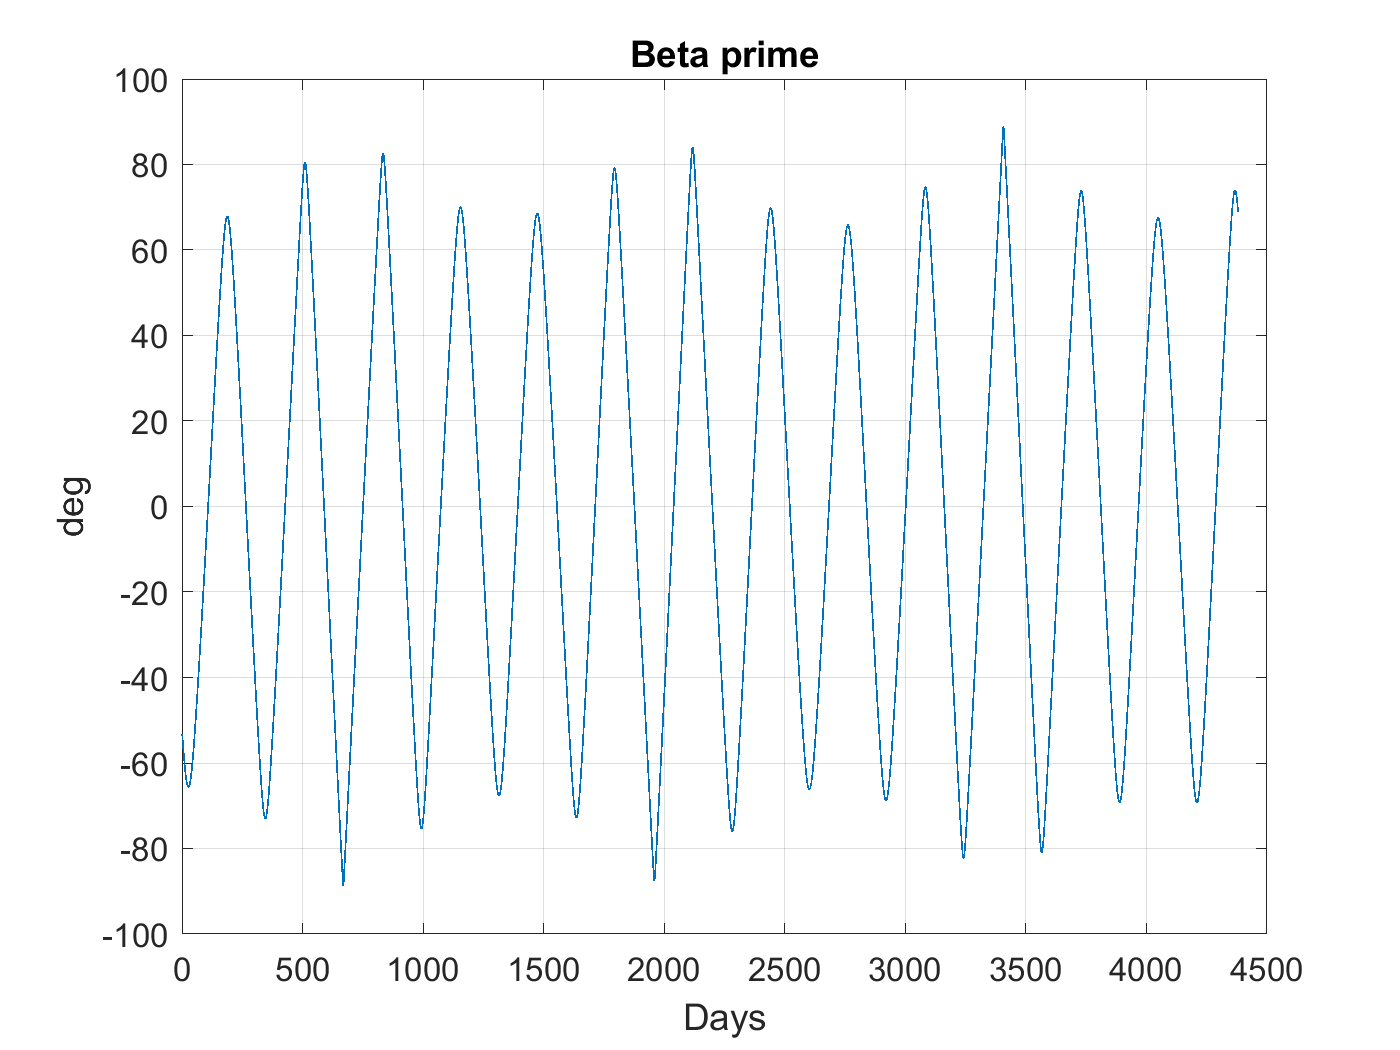
\includegraphics[width=0.8\textwidth]{beta_prime.png}
	\caption{$\beta ^\prime$ vs. time}
\end{figure}


\begin{enumerate}
	\item Is the variation of the $\beta ^\prime$ angle periodic? 
	\begin{itemize}
		\item Yes
	\end{itemize}
	\item Is the variation of the $\beta ^\prime$ angle sinusoidal? 
	\begin{itemize}
		\item Yes 
	\end{itemize}
	\item Why doesn't $\beta ^\prime$ angle in each cycle reach the same maximum value? 
	\begin{itemize}
		\item Because of orbital precession due to oblateness (like J2).
	\end{itemize}
\end{enumerate}



\newpage
% ================================================================ % 
\section*{Appendix} 

\subsection*{MATLAB code} 

\begin{lstlisting}
	%% ASE 387P.2 Mission Design HW 1 Junette Hsin 

	%% proficiency check 
	
	we = 7.292115e-5; % rad/s 
	
	% JD time (1999-01-21 20:43:47 UTC)
	JD1 = 2500000; 
	
	D = @(JD) JD - 2451545.0; 
	theta1 = 18.697374458 + 24.06570982 * D(JD1); 
	
	JD2 = JD1 + 1; 
	theta2 = 18.697374458 + 24.06570982 * D(JD2); 
	
	dtheta = theta2 - theta1; % hours 
	dtheta_deg = dtheta * 15; 
	we_deg = we * 60 * 60 * 24 * 180/pi; 
	
	sprintf('Proficiency check: accurate to %.9g', dtheta_deg - we_deg)
	sprintf('Confirmed Earth rotation rate is %.9g rad/s', we)
	
	%% problem 1 
	
	% Constants
	mu=3.986004415e14;
	ae=6378136.3;
	we=7.292115e-5;
	g=9.81;
	J2=1.082e-3;
	ws=1.99096871e-7;
	
	missions = {'Lageos', 'Topex', 'GRACE', 'ERS-1'}; 
	
	for i = 1:numel(missions)
		
		mission = missions{i}; 
		
		if isequal(mission,'Topex')
		a=7705;
		e=0.0010;
		I=65.99;
		end
	
		if isequal(mission,'GRACE')
		a=6820;
		e=0.0016;
		I=89.02;
		end
	
		if isequal(mission,'ERS-1')
		a=7156;
		e=0.0010;
		I=98.6;
		end
	
		if isequal(mission,'Lageos')
		a=12271;
		e=0.0040;
		I=109.83;
		end
	
		a=a*1000;
	
		% Orbital Rates
		nb=sqrt(mu/a^3);
	
		dOb=-3/2*nb*(ae/a)^2*J2*cosd(I)/(1-e^2)^(1/2);
		dwb=-3/4*nb*(ae/a)^2*J2*(1-5*cosd(I)^2)/(1-e^2)^2;
		dMb=nb*(1-3/4*(ae/a)^2*J2*(1-3*cosd(I)^2)/(1-e^2)^(3/2));
		dub=dwb+dMb;
	
		% Periods
		Tp=2*pi/nb;
		Ta=2*pi/dMb;
		Tn=2*pi/dub;
		TD=2*pi/(we+dOb);
		TS=2*pi/(ws+dOb);
		
		sprintf('Mission: %s', mission)
		sprintf('Keplerian period = %.5g', Tp)
		sprintf('Anomalistic period = %.5g', Ta) 
		sprintf('Draconitic period = %.5g', Tn)
		sprintf('Nodal day = %.5g', TD) 
		sprintf('Sun cycle = %.5g', TS) 
	
	end 

	%% Problem 2 

	clear 
	clc 

	JD=2457271.50000;
	n=JD-2451545;

	% n=5477.5+7442;

	L=280.46+0.9856474*n;
	Ll=floor(L/360);
	L=L-360*Ll;
	g=357.528+0.9856003*n;
	gg=floor(g/360);
	g=g-360*gg;

	lambda=L+1.915*sind(g)+0.02*sind(2*g); 
	B=0;
	e=23.439-0.0000004*n;
	a=atand(cosd(e)*tand(lambda));

	d=asind(sind(e)*sind(lambda));


	Thetag=18.697374458+24.06570982*(JD-2451545);
	Thetag=Thetag*15;
	Tg=floor(Thetag/360);
	Thetag=Thetag-360*Tg;

	Long=a-Thetag;
	Lat=d;

	if Long <-180
		Long=Long+180;
	end

	if Long >180
		Long=Long-180;
	end
	
	%% PROB 3
	
	clear
	clc
	
	% Constants
	mu=3.986004415e14;
	ae=6378136.3;
	we=7.292115e-5;
	g=9.81;
	J2=1.082e-3;
	ws=2*pi/365.2422/24/60/60;
	
	% orbit
	alt=350000;
	a=alt+ae;
	e=0;
	I=35;
	Long=+5.157;
	n=sqrt(mu/a^3);
	
	% O Precession Calcs
	sprintf('O precession:')
	Odot = -(3/2)*n*(ae/a)^2*J2*(1/(1-e^2)^(1/2))*cosd(I) % O precession
	
	sprintf('O precession for day:')
	Odotday = Odot*3600*24 % for day
	
	sprintf('Sun Precession for day:')
	wsd = ws*3600*24 % Sun Precession for day
	
	sprintf('Sun cycle period days:')
	Cs = 2*pi/(Odotday-wsd) % Sun Cycle period days
	
	sprintf('Clock time to decimal:')
	tc = 20+43/60+47/3600 % clock time to decimal
	
	sprintf('Local time at crossing TRMM:')
	LMTT = tc+(Long/15) % Local time at crossing TRMM
	
	sprintf('Local time Resurs')
	LMTR = 22+20/60 % Local time Resurs
	
	sprintf('Difference time between LMTT and LMTR:')
	time_diff = (LMTT-LMTR) % Difference time
	
	sprintf('Initial difference in time:')
	O_diff_change_day= 24/Cs %initial difference in time
	
	sprintf('Days since last cross: ')
	Offset = time_diff/(O_diff_change_day) % Days since last cross
	
	sprintf('Amount of crosses in 1 year:')
	k=0:round(abs(365.2425/Cs))-1 % amount of crosses in one year
	
	sprintf('offset by initial cross beforehand and set to cycle every Solar cycle:')
	Jk=round(21-Offset)+fix(k*abs(Cs)) % offset by initial cross beforehand and set to cycle every Solar cycle
	
	
	%% prob 4 
	
	h = 500e3;  % m  
	a0 = ae + h; 
	e0 = 0; 
	I0 = 89 * pi/180;     % rad
	w0 = 0; 
	long0 = 0; 
	M0 = 0; 
	
	% rv0 = oe2rv(0, [a0 e0 I0 w0 long0 nu0]); 
	
	%  Define parameters for a state lookup:
	% t0      = 'Oct 20, 2020 11:00 AM CST'; 
	t0      = 'May 22, 2018'; 
	abcorr  = 'NONE';
	
	%  Convert the epoch to ephemeris time (secs) 
	et_t0   = cspice_str2et( t0 );
	
	% get states --> Earth to Sun 
	target   = 'Sun';
	frame    = 'J2000';
	observer = 'Earth';
	abcorr   = 'NONE';
	
	% orbit rate equations 
	nb = @(a) sqrt(mu/a^3);
	dlongb = @(a, e, I) -3/2*nb(a)*(ae/a)^2*J2*cos(I)/(1-e^2)^(1/2);
	dwb = @(a, e, I) -3/4*nb(a)*(ae/a)^2*J2*(1-5*cos(I)^2)/(1-e^2)^2;
	dMb = @(a, e, I) nb(a)*(1-3/4*(ae/a)^2*J2*(1-3*cos(I)^2)/(1-e^2)^(3/2));
	dub = @(dwb, dMb) dwb+dMb;
	
	for k = 1 : 1 : 12*365 
	
		% delta time 
		dt = k * 60 * 60 * 24; 
		
		% rest of OEs 
		w(k,:)      = w0 + dwb(a0, e0, I0) * dt; 
		long(k,:)   = long0 + dlongb(a0, e0, I0) * dt; 
		M(k,:)      = M0 + dMb(a0, e0, I0) * dt; 
		
		% convert to cartesian 
		rv = oe2rv([a0, e0, I0, w(k,:), long(k,:), M(k,:)]); 
	%     rv = fn.orb2rv([a0, e0, I0, w(k,:), long(k,:), M(k,:)]); 
		
		% orbit plane 
		h = cross(rv(1:3), rv(4:6)); 
		h = h / norm(h); 
		
		% get sun position 
		et = et_t0 + dt;    % propagate ephemeris time by 1 day in secs 
		X_Esun  = spice_state(et, target, frame, abcorr, observer); 
		X_Esun  = X_Esun'; 
		r_sun   = X_Esun(1:3); 
		r_sun   = r_sun / norm(r_sun); 
		
		% get projection 
		sun_proj = dot(h, r_sun); 
		
		% Jonathan's method beta prime 
		b_prime(k,:) = 90 - acosd(sun_proj); 
		
	end 
	
	fname = 'beta prime'; 
	figure('name', fname); 
		plot(b_prime); 
		xlabel('Days') 
		ylabel('deg') 
		title('Beta prime') 
		
	sprintf('a. Q: Is the variation of the beta prime angle periodic?')
	sprintf('a. A: Yes')
	
	sprintf('b. Q: Is the variation of the beta prime angle sinusoidal?')
	sprintf('b. A: Yes')
	
	sprintf('c. Q: Why doesn't beta prime angle in each cycle reach the same maximum value?')
	sprintf('c. A: Because of orbital precession and other perturbing forces (like J2).')
	
	%% subfunctions 
	
	function rv = spice_state(epoch, target, frame, abcorr, observer) 
	
		rv = zeros(length(epoch), 6); 
		
		for i = 1:length(epoch) 
	
			%  Look-up the state for the defined parameters.
			starg   = mice_spkezr( target, epoch(i), frame, abcorr, observer);
			rv(i,:) = starg.state(1:6); 
			
		end 
	
	end 

	function [rv] = oe2rv(oe)
	% ------------------------------------------------------------------------ 
	% Purpose: Convert orbital elements and time past epoch to the classic 
	% Cartesian position and velocity
	% 
	% Inputs: 
	%   oe      = [6x1] or [1x6] orbital elements 
	%   delta_t = t - t0 time interval 
	%   mu      = Gravity * Mass (of Earth) constant 
	% 
	% Outputs: 
	%   rv      = position and velocity state vector 
	% ------------------------------------------------------------------------ 

	global mu 

	% orbital elements 
	a       = oe(1); 
	e       = oe(2); 
	i       = oe(3); 
	omega   = oe(4); 
	LAN     = oe(5); 

	%% the 6th element 
	M       = oe(6); 
	% M0      = oe(6); 
	% nu      = oe(6); 

	% nu is TRUE ANOMALY --> use Kepler's to calculate MEAN ANOMALY 
	% E = 2*atan( sqrt( (1-e)/(1+e) ) * tan(nu/2) ); 
	% M = M0 + sqrt( mu/a^3 ) * (delta_t); 
	%% 

	E = keplerEq(M, e, eps); 
	% E = kepler(M, e); 

	nu = 2*atan( sqrt( (1+e)/(1-e) ) * tan(E/2) ); 

	p = a * ( 1 - e^2 );            % intermediate variable 
	r = p / ( 1 + e*cos(nu) );      % r_magnitude, polar coordinates 

	% Perifocal position and velocity 
	r_pf    = zeros(3,1);  
	v_pf    = zeros(3,1); 
	r_pf(3) = 0; 
	v_pf(3) = 0; 
	r_pf(1) = r * cos(nu); 
	r_pf(2) = r * sin(nu); 
	v_pf(1) = -sqrt(mu/p) * sin(nu); 
	v_pf(2) = sqrt(mu/p) * (e + cos(nu)); 

	% Perifocal to ECI transformation, 3-1-3 rotation 
	R11 = cos(LAN)*cos(omega) - sin(LAN)*sin(omega)*cos(i); 
	R12 = -cos(LAN)*sin(omega) - sin(LAN)*cos(omega)*cos(i); 
	R13 = sin(LAN)*sin(i); 

	R21 = sin(LAN)*cos(omega) + cos(LAN)*sin(omega)*cos(i); 
	R22 = -sin(LAN)*sin(omega) + cos(LAN)*cos(omega)*cos(i); 
	R23 = -cos(LAN)*sin(i); 

	R31 = sin(omega)*sin(i); 
	R32 = cos(omega)*sin(i); 
	R33 = cos(i); 

	R = [R11 R12 R13; R21 R22 R23; R31 R32 R33]; 

	% Transform perifocal to ECI frame 
	r_vec = R * r_pf; 
	v_vec = R * v_pf; 

	% Position and state vector 
	rv = [r_vec; v_vec]; 

	end 

	%% Kepler equation solvers 

	function E = keplerEq(M,e,eps)
	% Function solves Kepler's equation M = E-e*sin(E)
	% Input - Mean anomaly M [rad] , Eccentricity e and Epsilon 
	% Output  eccentric anomaly E [rad]. 
		En  = M;
		Ens = En - (En-e*sin(En)- M)/(1 - e*cos(En));
		while ( abs(Ens-En) > eps )
			En = Ens;
			Ens = En - (En - e*sin(En) - M)/(1 - e*cos(En));
		end
		E = Ens;
	end

	function E = kepler(M, e)
		f = @(E) E - e * sin(E) - M;
		E = fzero(f, M);  % <-- I would use M as the initial guess instead of 0
	end
	
	
	
	
	
	
	
	
	
	
	
	
\end{lstlisting}





% ================================================================ % 

% \bibliography{sample}

\end{document}
